\documentclass[12pt]{article}
  \usepackage[francais]{babel}
  \AddThinSpaceBeforeFootnotes % à insérer si on utilise \usepackage[french]{babel}
  \FrenchFootnotes % à insérer si on utilise \usepackage[french]{babel}
  \usepackage[T1]{fontenc}
  \usepackage[utf8]{inputenc}
  \usepackage{graphicx}
  \usepackage[left=2.5cm,right=2.5cm,top=2.5cm,bottom=2.5cm]{geometry}
  \usepackage{array}
  \usepackage{booktabs}
  \usepackage[squaren,Gray]{SIunits}  % Unité ex: $\unit{5 \cdot 10^{-6}}{\meter}$
  \usepackage{colortbl}               % Pour les couleur des cellules (tableau)
  \usepackage{amsmath}				  % Pour les formules mathématiques
  \usepackage{upgreek}                % Pour les lettres greque
  %\usepackage{fullpage}	          % plus petites marges
  \usepackage{verbatim}				  % Pour de long commentaires
  \usepackage[lofdepth,lotdepth]{subfig}       % Faire des sous-figures
  \usepackage{url}
  \usepackage{colortbl}               % pour les couleur des cellules (tableau)
  \usepackage{indentfirst}
  \usepackage{multirow}
  \usepackage{xfrac}
  \usepackage{wrapfig}
  \usepackage{enumitem}               % Liste personnalisée
  \frenchbsetup{StandardLists=true}   % Empêche conflits entre enumitem et babel
  \usepackage{placeins}   % place une barrière pour que l'image/table soit derrière \FloatBarrier
  \usepackage{lastpage} 
  \usepackage{titling}
  \usepackage{lmodern}
  \usepackage{booktabs}
  \usepackage{etoolbox}
  \usepackage[most]{tcolorbox}
  
  
  %Change la taille de police
  \newcommand\ChangeRT[1]{\noalign{\hrule height #1}}
  
\graphicspath{{images/}}

  
  %Création  d'une nouvelle commande pour faire référence à une Figure
  %Exemple : \appelFigure{schema} donne : Figure 1 (en italique)
  \newcommand{\appelFigure}[1]{
    \textit{Figure \ref{#1}}
  }
      
  %%Création commande pour insérer image avec nom de figure directement
  %\newcommand{nomDeTaCommande}[nombreArguments]{CodeLaTeX}
  %\insertImage[position]{image_path}{scale}{Titre_figure}{label}
  \newcommand{\insertImage}[5][center]{
      \begin{#1}
      \includegraphics[scale=#3]{#2}
      \captionof{figure}{#4} 
      \label{#5}
      \end{#1}
  }

  % Affichage des frames pour commande cisco
  \newtcblisting{cisco}[1][]{size=fbox, listing only, listing options={style=tcblatex,basicstyle=\ttfamily\scriptsize,tabsize=2,language=sh},title=#1}

  %En-tête et pied de page personalisé
  \usepackage{fancyhdr}
  \pagestyle{fancy}
  \fancyhf{}
  \setlength\parindent{0pt} %Supprime les alinéa
  \setlength{\parskip}{8pt} %Augmente l'espace entre paragraphe
  %Bottom numbering page
  \renewcommand{\headrulewidth}{1pt}
  \fancyhead[L]{
\includegraphics[scale=.2]{heia-fr-logo.png}}
  \fancyhead[R]{\theauthor}
  
  \renewcommand{\footrulewidth}{1pt}
  \fancyfoot[R]{\textbf{Page \thepage\ sur \pageref{LastPage}}} 
%  \fancyfoot[L]{\leftmark}

  \setlength\parindent{0pt} %Supprime les alinéa
  \setlength{\parskip}{8pt} %Augmente l'espace entre paragraphe


\title{Système Embarqués II, Journal, TP.05\\  Introduction au langage assembleur et interface avec le C}
\author{\textsl{Marc} \textsc{Roten} \\ \textsl{Sven} \textsc{Rouvinez}}
\date{}

\begin{document}
    \begin{titlepage}
        \begin{center}
            
\includegraphics[scale=.3]{heia-fr-logo.png}\\[1.3cm]
            
            \rule{\linewidth}{0.3mm} \\[0.3cm]
            {\huge \bfseries Système embarqués \\[0.5cm]} 
            \rule{\linewidth}{0.3mm} \\[0.8cm]
            \noindent
            \begin{minipage}[t]{0.4\textwidth}
                \begin{flushleft} \large
                    \emph{Auteurs :}\\
                    \theauthor
                \end{flushleft}
            \end{minipage}
            \begin{minipage}[t]{0.4\textwidth} 
                \begin{flushright} \large
                    \emph{Professeur:}\\
                    \textsl{Daniel} \textsc{Gachet}\\ 
                \end{flushright} 
                \vfill
            \end{minipage}\\[1.3cm]
            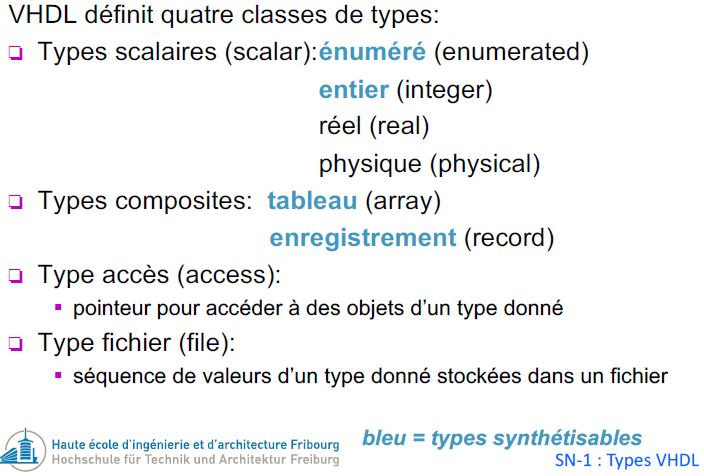
\includegraphics[scale=0.6]{1.JPG}\\[1.5cm]
            \vspace*{1\baselineskip}
            \today \\[0.7cm]
        \end{center}
    \end{titlepage}
    \tableofcontents
    \clearpage
% \insertImage{Img/1.PNG}{echelle pour l'image (source = 1)}{texte dessous l'image}{référence vers l'objet}
\section{Heure de travail}
12 heures

\section{Introduction}
Dans ce travail nous allons réaliser notre premier TP en assembleur en réalisant une tour de Hanoi.
\section{Synthèse}

\paragraph{Sven}

\textbf{\textit{Acquis}}
\begin{itemize}
    \item Appel de fonction en assembleur
    \item Passage de paramètres
    \item Sauvegarde des registres et restauration
\end{itemize}

\paragraph{Marc}

\textbf{\textit{Acquis}}
\begin{itemize}
    \item Programmation en assembleur
    \item Debuggage assembleur
    \item Utilisation du Display du beaglebone
    \item Sauvegarde de registre et appel de fonction
\end{itemize}


\newpage
\section{Question}

\textbf{Pour les deux structures struct S1 et struct S2 et le code ci-dessous? indiquez la convention utilisée pour: }


\begin{lstlisting}
    struct S1 {int a;};
    struct S2 {int a; int b[100];};
    
    struct S1 f1();
    struct S2 f2();
    
    void f3 (int a, int b, int c, int d, struct S2 s);
    void f4 (int a, int b, int c, int d, const struct S2* s);
    void f5 (struct S2 s, int a, int b, int c, int d);
    void f6 (const struct S2* s, int a, int b, int c, int d);
    void f7 (struct S1 s);      
\end{lstlisting}

\begin{lstlisting}
    void main(){
    //point 1
    struct S1 r1 = f1();
    struct S2 r2 = f2();

    //point 2
    f3 (12,43,16,19,S2);
    f4 (76,33,11,22,S2);
    f5 (S2,11,22,33,44);
    f6 (&S2,99,88,77,66);
    f7 (&S1);
    }   
\end{lstlisting}

\begin{enumerate}
    \item Le retour de ces structures par les fonctions f1 et f2
       \begin{itemize}
          \item \texttt{f1()} Retourne uniquement un int contenu dans la structure S1, donc un seul registtre suffit et sera retournée par lui même
          \item \texttt{f2()} Retourne un int et un tableau contenant 100 int. Un registre est limité à 32 bit donc il faudra retourne une adresse qui pointe sur la stack qui elle contient les 101 int
       \end{itemize}
    \item Le passage par valeur de ces structures par les fonctions f3 à f7: les 4 premiers arguments sont donnés par les registres r0 à r3, et s'il y a plus de 4 arguments ils doivent être passés par la pile
       \begin{itemize}
          \item \texttt{f3()} les 4 premiers int seront passés par les registres r0 à r3 et la struct sera passé par la pile
          \item \texttt{f4()} les 4 premiers int seront passés par les registres r0 à r3 et le dernier argument est un pointeur constant sur la struct S2 et l'adresse est donnée par la pile

          \item \texttt{f5()} le passage des paramètres est mal agencé ici car la structure prend de la place et ne peut donc pas être placée dans le registre 0, par contre pour les autres paramètres il sera possible de les passer par les registres et un par la pile

          \item \texttt{f6()} étant donné que la structure est un pointeur et une constante, le registre 0 contiendra uniquement l'adresse, les 3 autres par les registres r1 r2 et r3 et le dernier par la pile

          \item \texttt{f7()} le seul argument est la structure S1 et elle contient uniquemement un int donc elle peut être passée par le r0 mais cela n'est pas optimal, par contre il ne sera pas possible de modifier la structure dans d'autres méthodes vu qu'elle est passé par copie et donc cela limite les effets de bords
       \end{itemize}
\end{enumerate}

 
\section{Conclusion}
Ce TP était intéressant, il nous a permis de comprendre comment traduire une série de fonction en assembleur et de pouvoir comprendre comment passer des paramètres ainsi que l'écriture de fonctions récursive.
On a aussi pu constater que la taille (en byte) d'un fichier assembleur était bien moindre que la taille d'un fichier C. Ce qui est non-négligable pour des systèmes embarqués

\end{document}
